\documentclass[10pt,letterpaper]{article}
\usepackage[utf8]{inputenc}
\usepackage{geometry}
\geometry{margin=0.75in}
\usepackage{titlesec}
\usepackage{enumitem}
\usepackage{hyperref}
\usepackage{xcolor}
\usepackage{fontawesome}
\usepackage{graphicx}
\usepackage{calligra} % For signature-style font
\definecolor{headercolor}{RGB}{0, 102, 204}
\definecolor{subheadercolor}{RGB}{51, 51, 51}

% Formatting for section headers
\titleformat{\section}{\large\bfseries\color{headercolor}}{\thesection}{1em}{}
\titleformat{\subsection}{\normalsize\bfseries\color{subheadercolor}}{\thesubsection}{1em}{}

% Custom commands
\newcommand{\entry}[4]{\textbf{#1} \hfill #2 \\ \textit{#3} \hfill #4 \\}
\newcommand{\project}[3]{\textbf{#1} \hfill #2 \\ \textit{#3} \\}

% Remove default page numbers
\pagestyle{empty}

\begin{document}

\begin{center}
    % Profile picture placeholder
    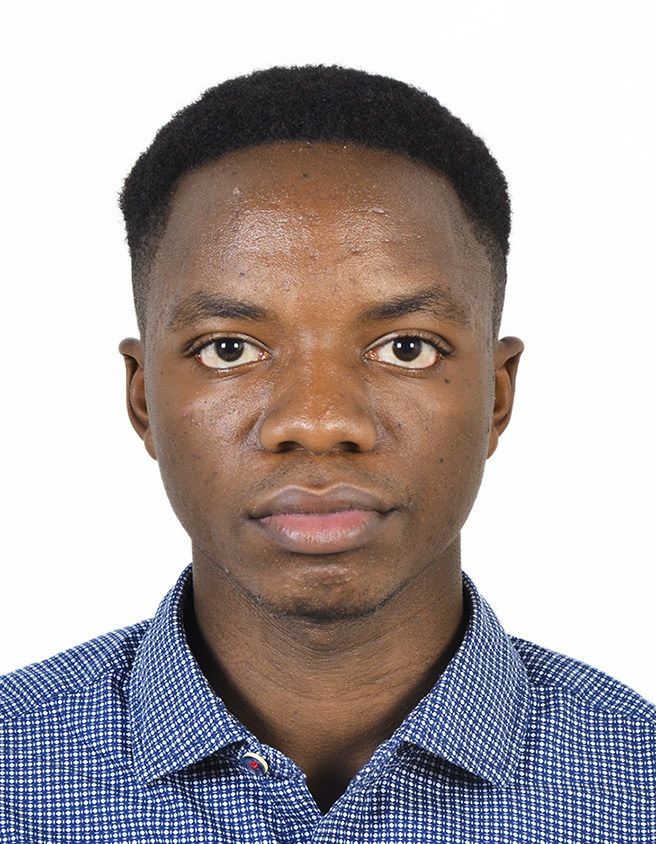
\includegraphics[width=3cm, height=8cm, keepaspectratio]{tony.JPG} \\[0.2cm]
    {\Huge \textbf{Tony Blaise Bimenyimana}} \\[0.2cm]
    Lioning, Shenyang, China | \faPhone~+86 188 0407 2112 | \faEnvelope~\href{mailto:tonyblaisb@gmail.com}{tonyblaisb@gmail.com} \\
    \faLinkedin~\href{https://www.linkedin.com/in/tony-blaise-bimenyimana}{Tony Blaise Bimenyimana} | \faGithub~\href{https://github.com/TonyBimenyi}{TonyBimenyi} \\[0.2cm]
\end{center}

\section*{Objective}
Motivated researcher and software engineer with a Bachelor’s in Software Engineering and a Master’s in Automatic Control and Electrical Engineering (in progress). Seeking opportunities to apply expertise in data-driven control, web development, and graphic design to innovate and deliver impactful solutions in technology and automation.

\section*{Education}
\entry{Master of Science in Automatic Control and Electrical Engineering}{Sep 2023 -- Present}
{Shenyang Aerospace University}{Shenyang, China}
\begin{itemize}[leftmargin=*,nosep]
    \item Research Focus: Data-Driven Control Systems
    \item Achievements: 1st and 3rd Place in University Photo Contest (2024)
\end{itemize}

\entry{Bachelor of Science in Software Engineering}{Sep 2020 -- Dec 2022}
{Bujumbura International University}{Bujumbura, Burundi}
\begin{itemize}[leftmargin=*,nosep]
    \item Relevant Coursework: Web Development, Algorithms, Database Systems
    \item Certifications: GDSC-BIU Member, English Language Certification
\end{itemize}

\section*{Work Experience}
\entry{Website Developer \& Graphic Designer}{Dec 2019 -- Dec 2023}
{HOGI Burundi Company}{Bujumbura, Burundi}
\begin{itemize}[leftmargin=*,nosep]
    \item Developed and maintained websites including \href{https://hogi.bi}{hogi.bi} and \href{https://ifb-burundi.bi}{ifb-burundi.bi}, enhancing user experience and accessibility.
    \item Designed a web application for Burundi Free Methodist Church to manage employee pension funds, streamlining administrative processes.
    \item Created marketing materials using Adobe Photoshop, Illustrator, Premiere Pro, and After Effects, boosting client engagement by 20\%.
\end{itemize}

\section*{Projects}
\project{Employee Pension Fund Web Application}{2022}{Burundi Free Methodist Church}
\begin{itemize}[leftmargin=*,nosep]
    \item Built a secure web platform using Laravel and Vue.Js to automate pension fund management, reducing processing time by 30\%.
    \item Integrated user-friendly interfaces with HTML, CSS, and JavaScript for seamless navigation and laravel APIs.
\end{itemize}

\project{HOGI Website Development}{2021 -- 2023}{HOGI Burundi}
\begin{itemize}[leftmargin=*,nosep]
    \item Led front-end and back-end development for \href{https://hogi.bi}{hogi.bi} using Django and DRF, improving site performance and SEO rankings.
    \item Designed visually appealing graphics with Adobe Illustrator and Affinity Photo 2.
\end{itemize}

\section*{Skills}
\begin{itemize}[leftmargin=*,nosep]
    \item \textbf{Technical}: Python, MATLAB, HTML, CSS, JavaScript, Laravel, PHP, Django, DRF, Vue.JS, Ionic, Java, Android Studio, C, C++, Control Systems, Adobe Photoshop, Adobe Illustrator, Adobe Premiere Pro, Adobe After Effects, Affinity Photo 2
    \item \textbf{Soft Skills}: Team Collaboration, Problem-Solving, Communication
    \item \textbf{Certifications}: GDSC-BIU Member, English Language Certification
\end{itemize}

\section*{Languages}
\begin{itemize}[leftmargin=*,nosep]
    \item Kirundi (Native), English (Fluent), French (Fluent), Swahili (Fluent), Kinyarwanda (Fluent), Chinese (Basic)
\end{itemize}

\section*{Additional Information}
\begin{itemize}[leftmargin=*,nosep]
    \item \textbf{Born}: May 24, 2002
    \item \textbf{Interests}: Photography, Open-Source Development, Data-Driven Research
\end{itemize}

\section*{Declaration}
I hereby declare that all the information provided in this resume is true and accurate to the best of my knowledge.

\vspace{0.5cm}
{\calligra \large Bimenyimana Tony Blaise} \\
\textit{Signature}

\end{document}